%%%% ijcai11.tex

\typeout{IJCAI-11 Instructions for Authors}

% These are the instructions for authors for IJCAI-11.
% They are the same as the ones for IJCAI-07 with superficical wording
%   changes only.

\documentclass{article}
% The file ijcai11.sty is the style file for IJCAI-11 (same as ijcai07.sty).
\usepackage{ijcai11}
\usepackage{mathtools}
\usepackage[utf8]{inputenc}

% For importing images.
\usepackage{graphicx}

% The language we want and appropriate hyphenation.
\usepackage[dutch]{babel}

% Hyphenation rules.
\hyphenation{biopotentiaal-schommelingen}

% Use the postscript times font!
\usepackage{times}

% the following package is optional:
%\usepackage{latexsym} 


\title{TODO Titel}
\author{Kevin Boets \\ Katholieke Universiteit Leuven\\ Leuven, Belgium \\ kevin.boets@student.kuleuven.be
\And
Gertjan Franken \\ Katholieke Universiteit Leuven\\ Leuven, Belgium \\ gertjan.franken@student.kuleuven.be}

\begin{document}

\maketitle

\begin{abstract}
 TODO
  The {\it IJCAI--11 Proceedings} will be printed from electronic
  manuscripts submitted by the authors. The electronic manuscript will
  also be included in the online version of the proceedings. This paper
  provides the style instructions.
\end{abstract}

\section{Introductie}

TODO 

\section{Preprocessing}

De data die we krijgen doorgestuurd, afkomstig van de sensoren, is zeer ruw. Om hier kijkrichtingen uit af te kunnen leiden, gaan we de data eerst beter leesbaar maken. Dit is de preprocessing-stap. Deze stap voeren we uit op elke dataset,  alvorens we deze gaan analyseren. Beschouw de data in figuur 1 als de originele data.

\begin{figure}[h]
\centering
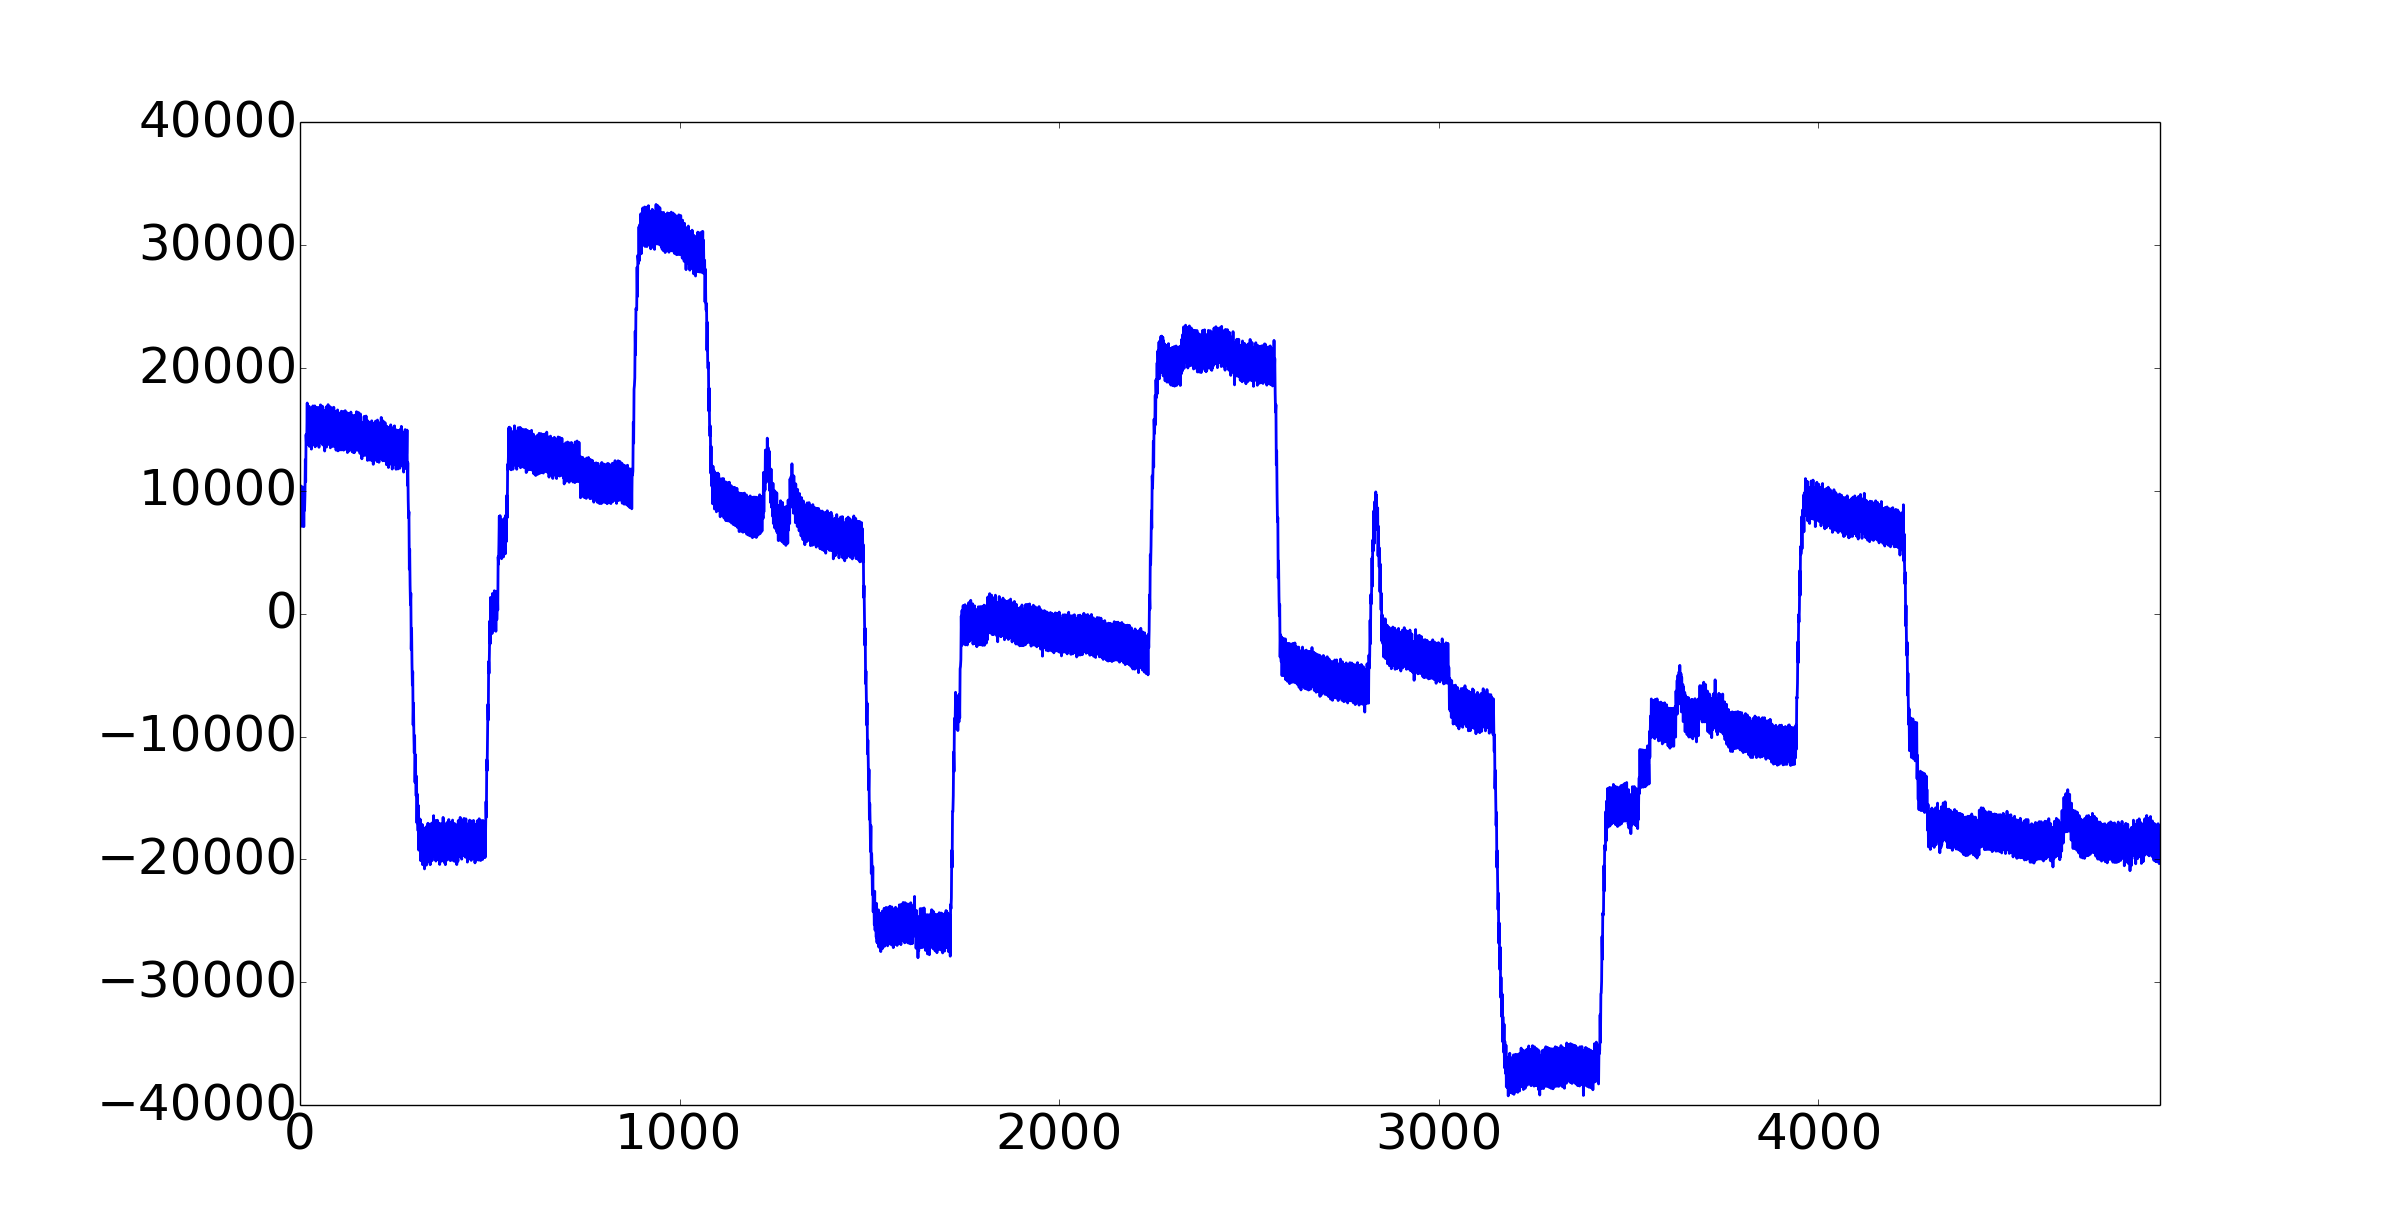
\includegraphics[width=\linewidth]{images/original_data}
\caption{Originele data rechtstreeks afkomstige van de hardware.}
\end{figure}

Als eerste gaan we de ruis en knipperingen zo goed mogelijk proberen te verminderen. Dit gebeurt door middel van een low-pass filter. Deze filter verzacht alle signalen waarvan de frequentie hoger is dan onze cutoff frequentie. [TODO berekenen wat onze cutoff frequentie is].

Daarna focussen we ons op de biopotentiaalschommelingen. Deze schommelingen kunnen we niet op voorhand voorspellen en verschillen van persoon tot persoon. Als we deze schommelingen kunnen verminderen, kunnen we meer steunen op absolute waardes van het signaal. In dit tweede deel van de preprocessing-stap gebruiken we opnieuw een low-pass filter. Deze keer gebruiken we een lage cutoff frequentie [TODO weer cutoff berekenen]. Na deze filtering van de data, blijven enkel de signalen met een lage frequentie over. Het resultaat is ongeveer de biopotentiaal van de gebruiker die doorheen de tijd fluctueert. We kunnen nu de biopotentiaalschommelingen uit onze originele data verminderen door de gevonden biopotentiaal hiervan af te trekken. De schommelingen verdwijnen niet volledig, maar worden wel sterk verminderd.

\begin{figure}[h]
\centering
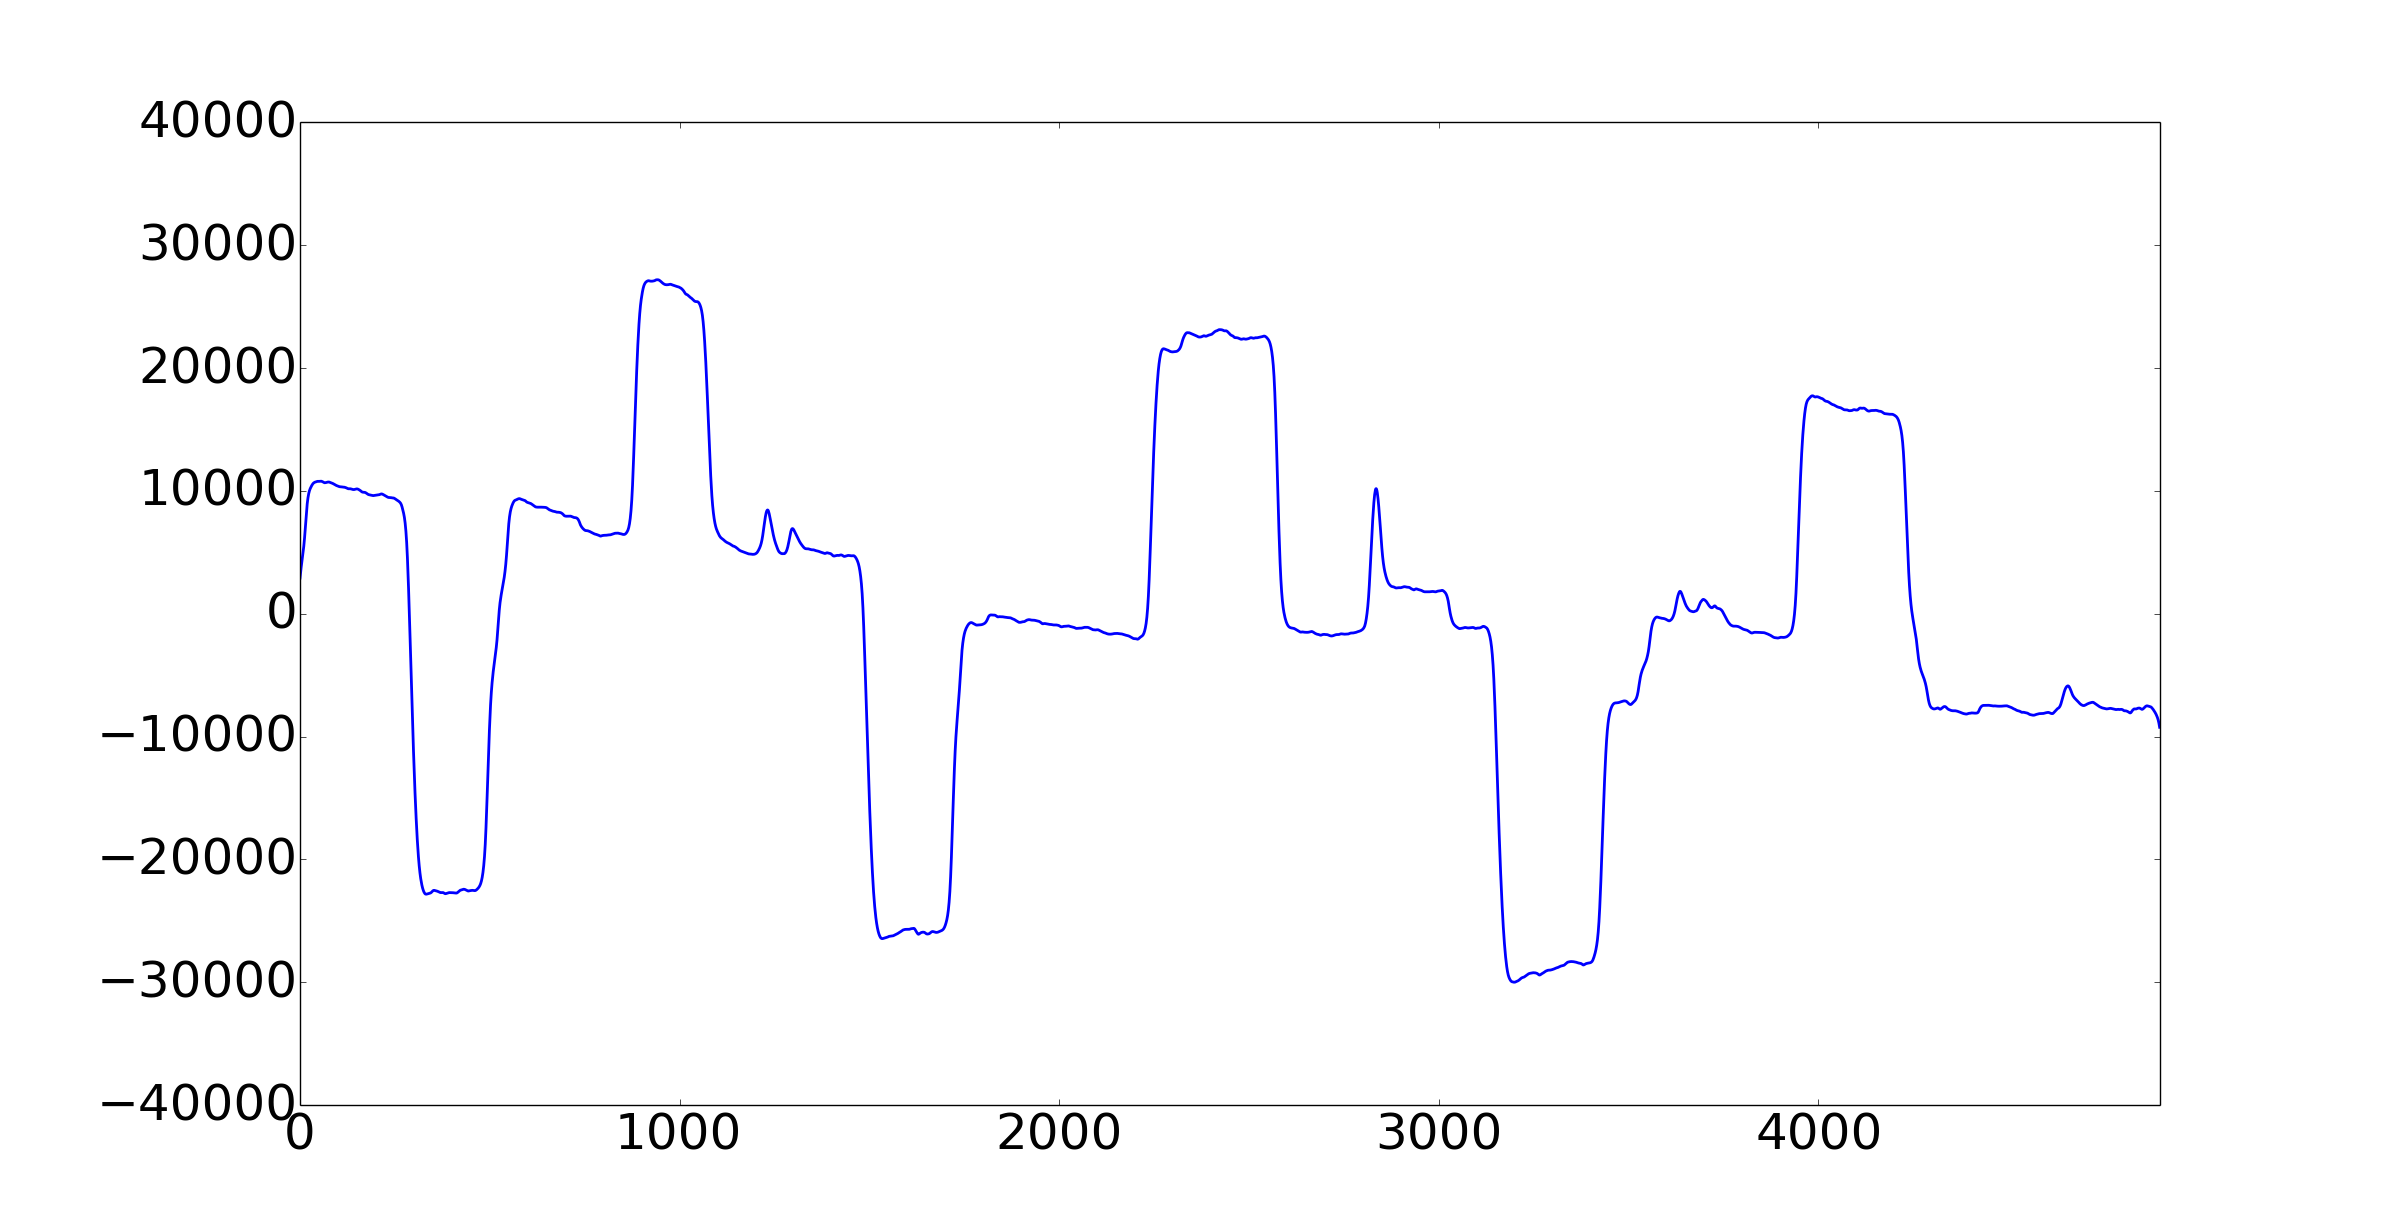
\includegraphics[width=\linewidth]{images/filtered_data}
\caption{Het resultaat van de twee filteringen op de originele data. De ruis is sterk verminderd en de sterkte van de knipperingen is afgenomen. De biopotentiaalschommeling is niet helemaal weg, maar wel voldoende verminderd.}
\end{figure}

Na toepassing van de vorige filteringen, discretiseren we de data. Hierdoor moeten we later minder berekeningen doen, wat de uitvoeringstijd van het programma ten goede komt. Hiervoor gebruiken we SAX (Symbolic Aggregate approXimation) \cite{sax}. De verdeling van de letters die het SAX-woord opmaken, bepalen we op de volgende manier. Om een goede verdeling te hebben, moeten de letters ongeveer even veel voorkomen. Eerst worden alle punten van de dataset gesorteerd op waarde, van klein naar groot. We verkrijgen hierdoor dus een stijgende grafiek. Afhankelijk van de alfabetgrootte $a$ (het aantal letters dat we gebruiken), verdelen we deze grafiek in even veel verrschillende partities die elk dezelfde grootte hebben. Daarna wordt elke letter uit ons alfabet aan een van die partities gekoppeld. Eigenlijk heeft elke letter nu een interval. We definiëren ook op voorhand hoeveel waarden een letter voor moet stellen. Dit is de constante $w$. De data die we willen discretiseren, verdelen we op een partities van lengte $w$. Voor elke partitie berekenen we het gemiddelde. We kennen een letter toe aan zo een partitie afhankelijk van dit gemiddelde.[TODO beter verwoorden en rest SAX (zoals letterwaarden)] [TODO nieuwe verdeling]

\begin{figure}[h]
\centering
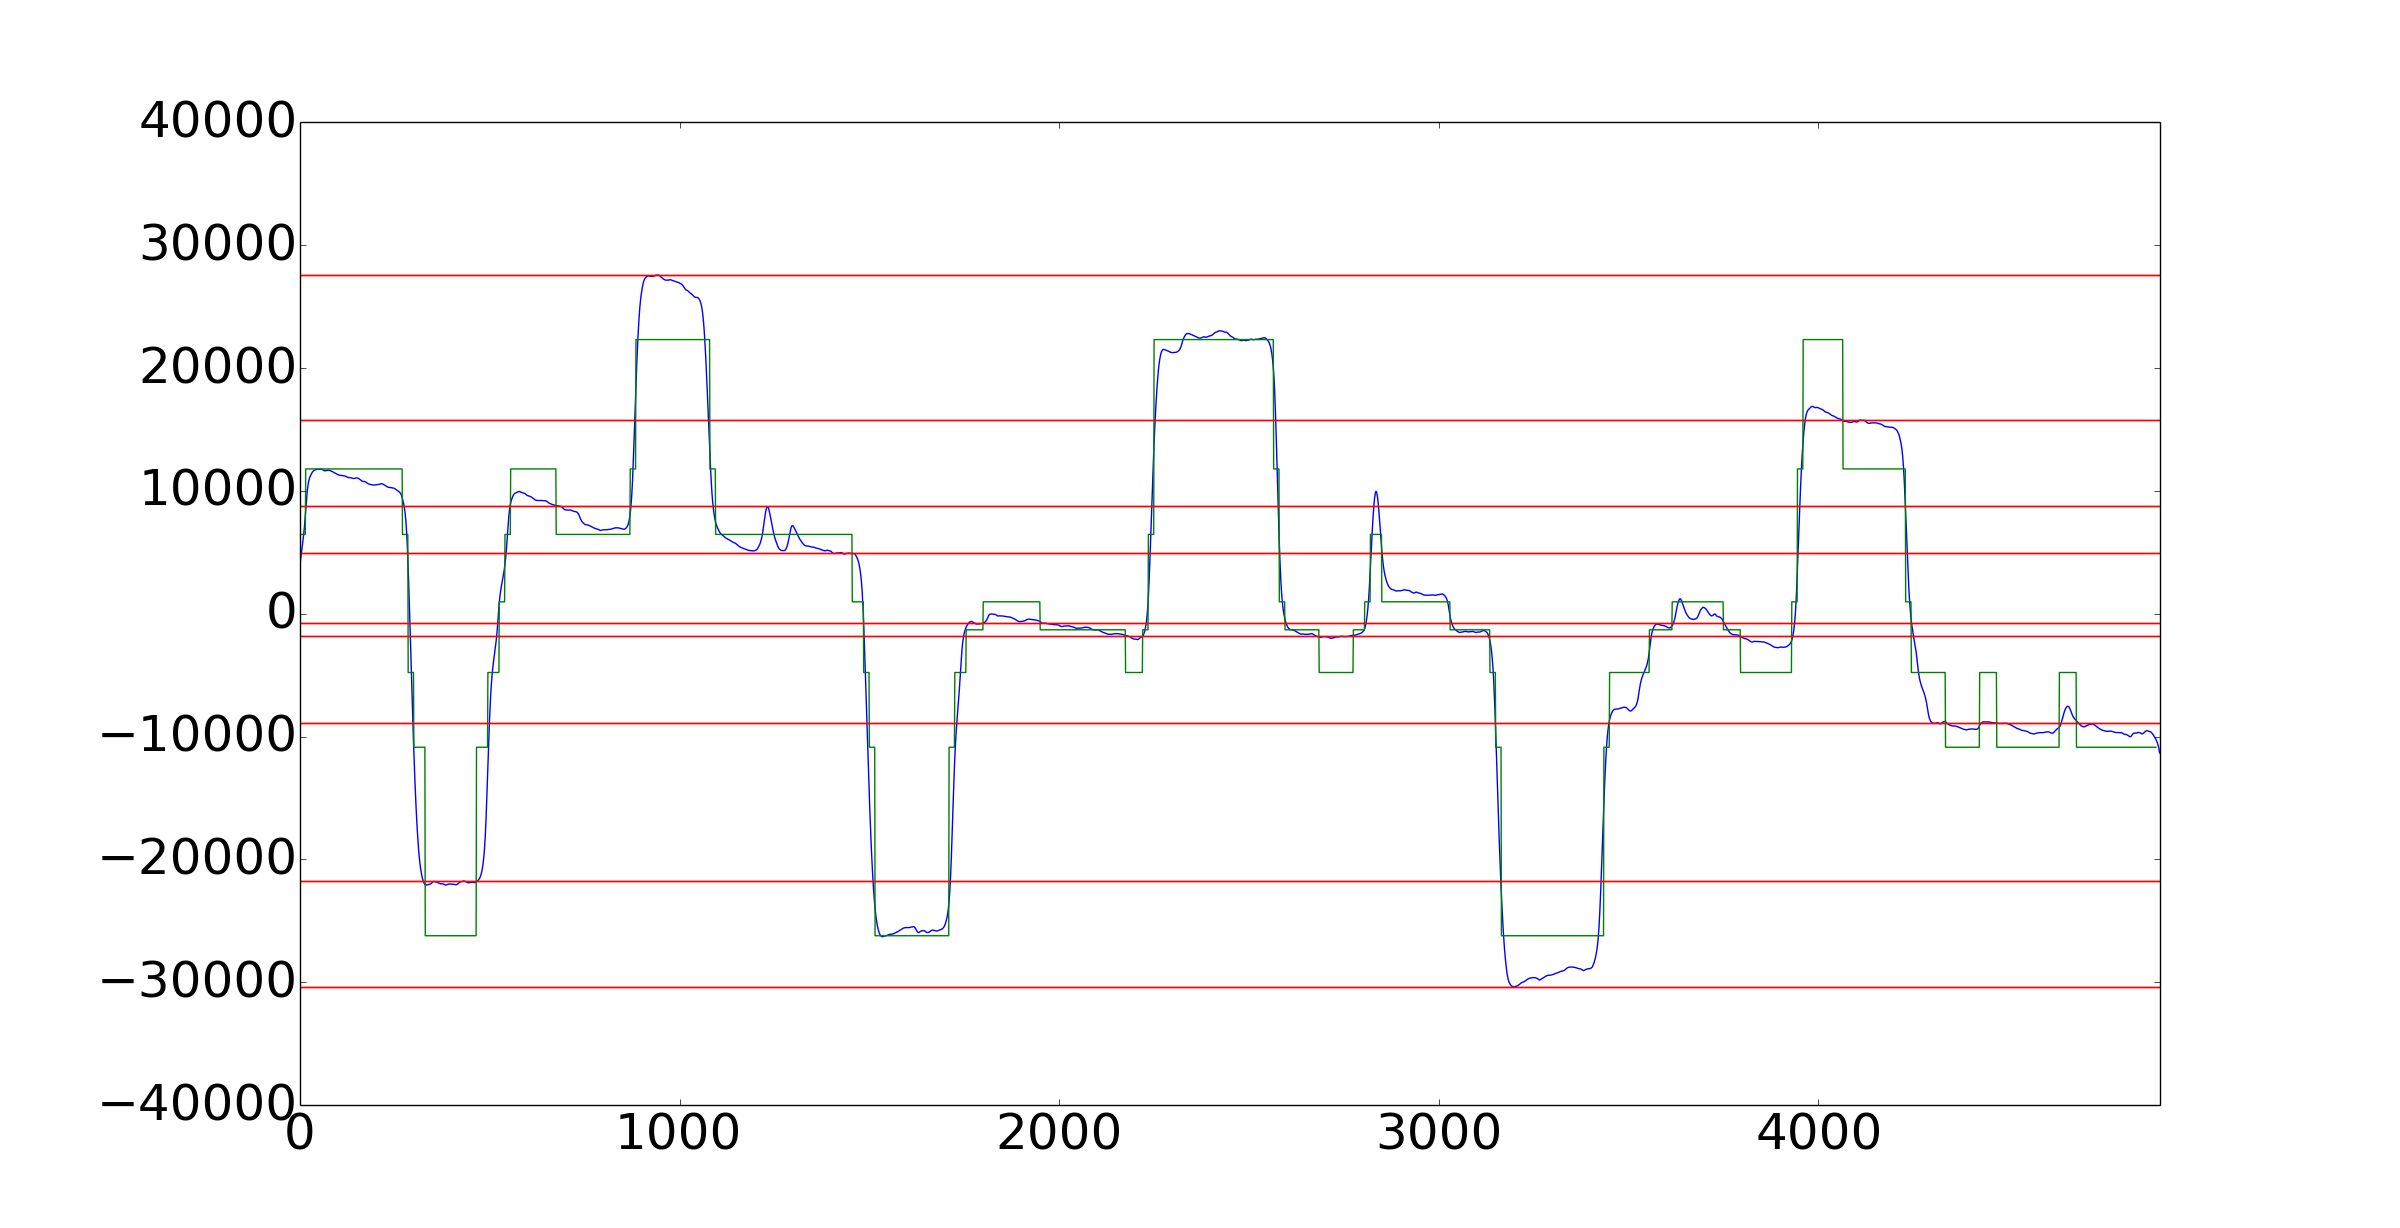
\includegraphics[width=\linewidth]{images/discretized_data}
\caption{De groene lijn stelt de discretisatie voor van de gefilterde data die in het blauw staat. De rode horizontale lijnen geven de distributie weer van de SAX-letters.}
\end{figure}

[TODO nog een afbeelding met enkel de groene lijn?]
[TODO slot?]

\section{Gebruikte methoden}

In ons onderzoek hebben we gebruik gemaakt van twee verschillende methoden om kijkrichtingen te herkennen. Deze methoden steunen respectievelijk op thresholds en patronen. Beide methoden beginnen met een calibratie-fase, gevolgd door een herkennings-fase. In de calibratie-fase laten we de gebruiker naar een aantal richtingen kijken, waarna we deze data analyseren. De gevonden informatie koppelen we aan de juiste kijkrichting. In de herkennings-fase wordt deze informatie gebruikt om in de nieuwe data kijkrichtingen te detecteren.

\subsection{Thresholds}

Deze methode steunt op de absolute waarden van de data. Er wordt een bovengrens gedefinieerd voor elke kijkrichting in de calibratie-fase. Als deze overschreden wordt in de herkennings-fase, gaan we uit van die bepaalde kijkrichting.

In de calibratie-fase wordt aan de gebruiker gevraagd om een bepaalde sequentie van kijkrichtingen uit te voeren. Uit deze dataset halen we de kleinste en grootste waarde. Deze twee waarden horen elk bij een andere kijkrichting. Per kijkrichting hebben we ook een constante $\alpha$ waarvoor geldt: $0 < \alpha \leq 1$. We vermenigvuldigen $\alpha$ met dit minimum en maximum en beschouwen de uitkomsten als de uiteindelijke bovengrens van de respectievelijke kijkrichtingen. In ons programma hebben we $\alpha$ voor beide kijkrichtingen de waarde $0.5$ gegeven, maar deze kan veranderd worden naar behoefte. Zo kunnen we de methode bijvoorbeeld strenger maken door $\alpha$ te verhogen. [TODO vemelden welke $\alpha$ wij gebruiken]

\begin{figure}[h]
\centering
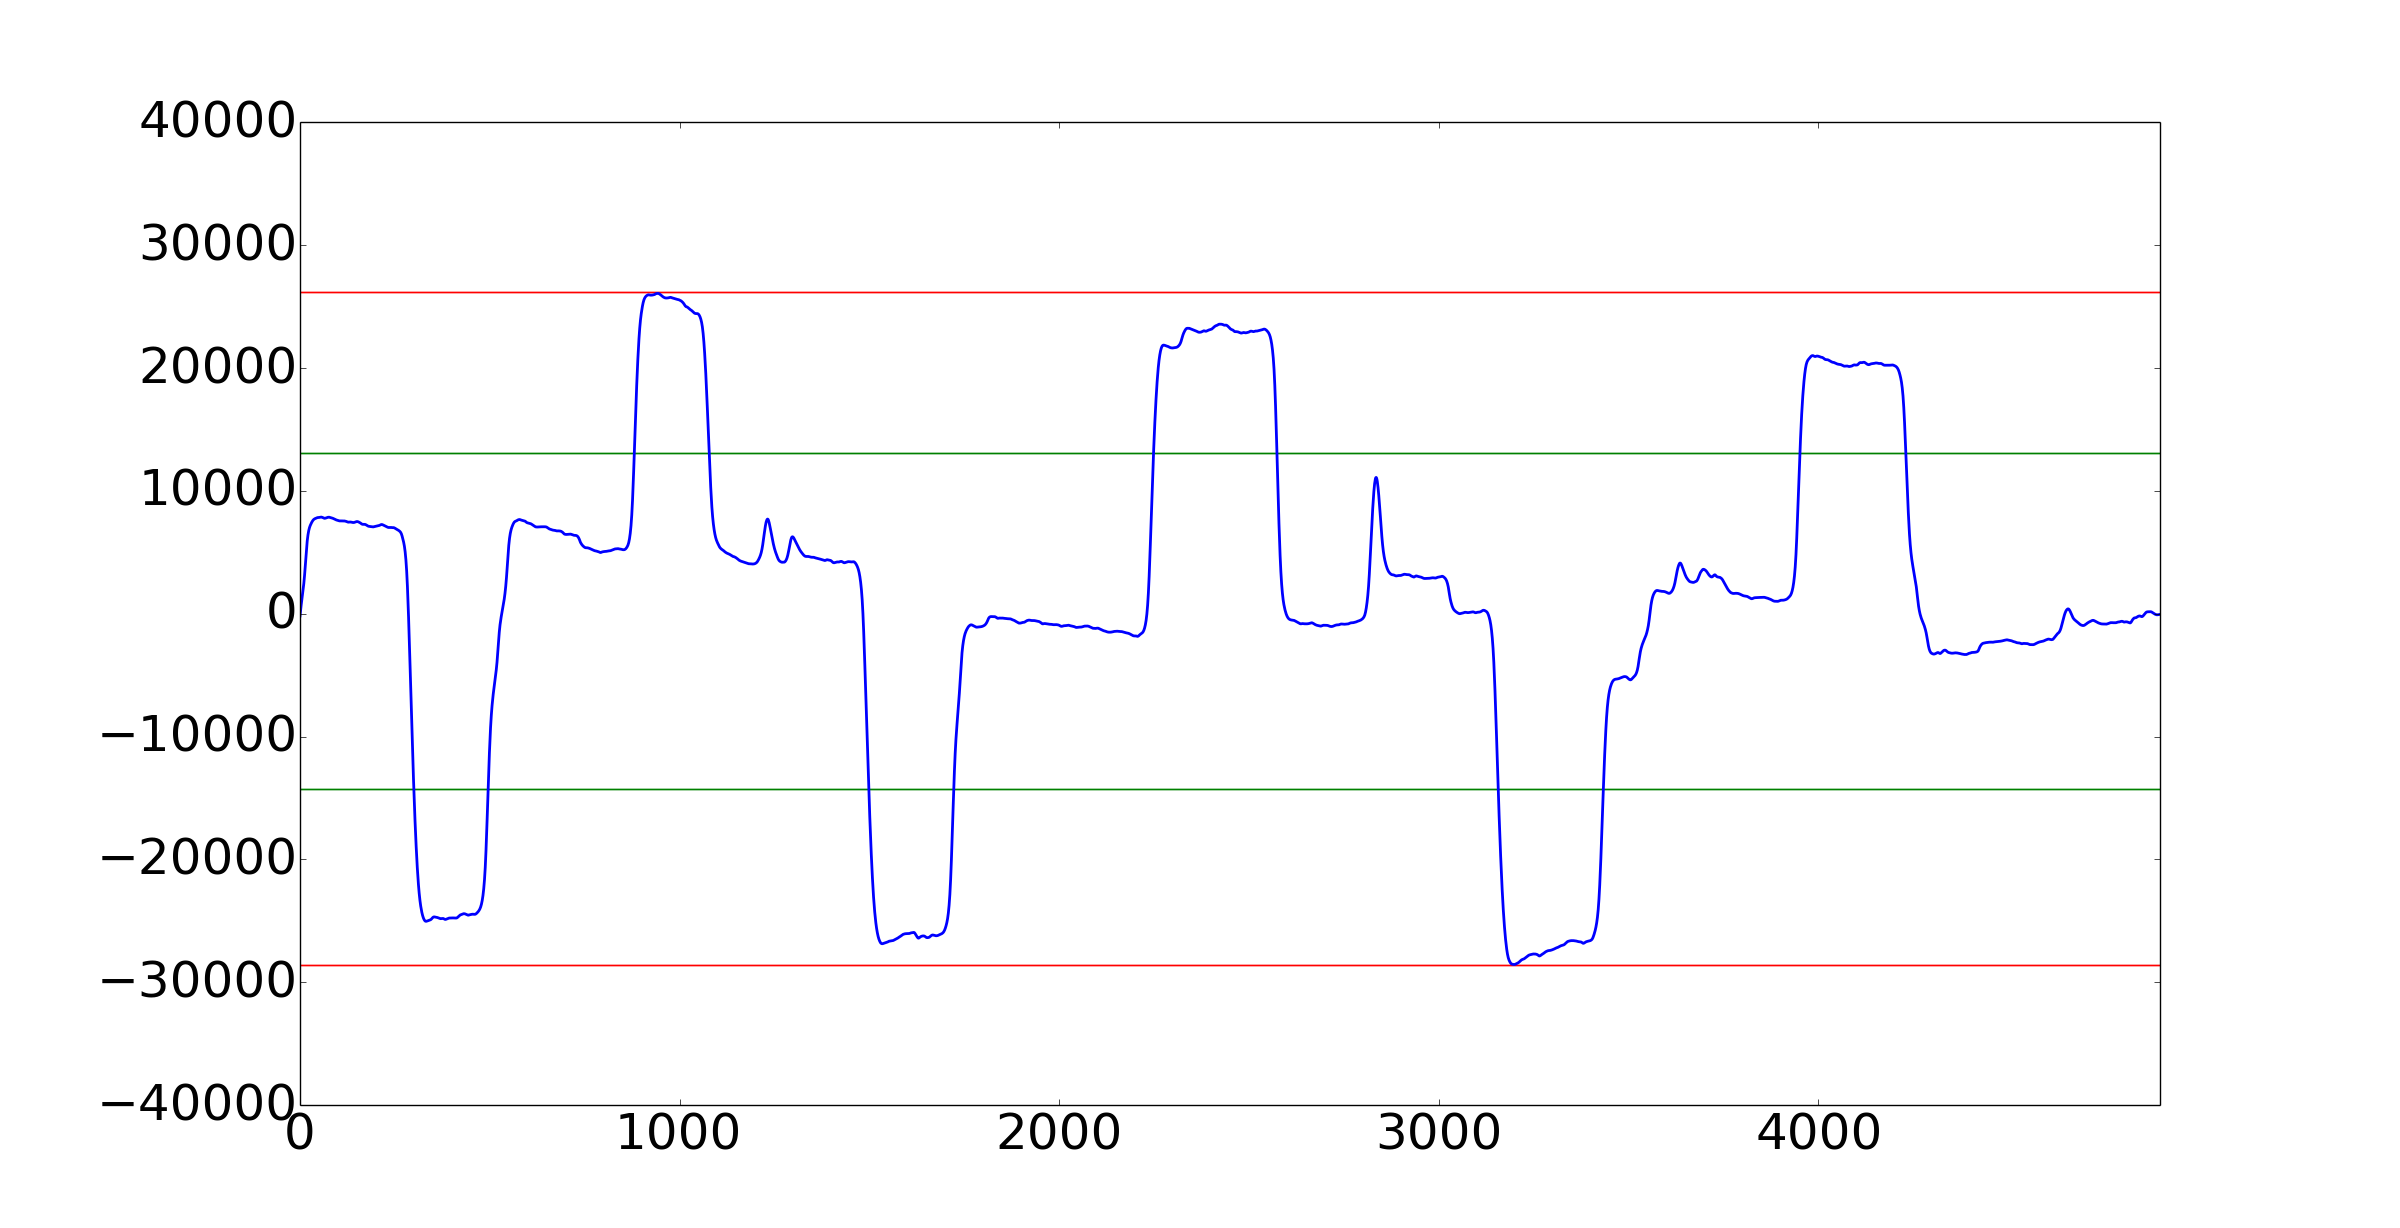
\includegraphics[width=\linewidth]{images/thresholds_distribution}
\caption{In deze afbeelding stellen de rode lijnen het minimum en maximum voor. De groene lijnen zijn het minimum en maximum vermenigvuldigd met $\alpha$.}
\end{figure}

In de herkennings-fase gaan we met behulp van deze bovengrenzen kijkrichtingen proberen te detecteren. We nemen telkens het gemiddelde van tien nieuwe punten. Dit gemiddelde gaan we dan vergelijken met alle bovengrenzen. Wanneer een bovengrens overschreden wordt, toont dit aan dat de gebruiker mogelijk in een van de richtingen aan het kijken is. Dit is echter niet altijd zo. Een paar opeenvolgende pieken in de data (zoals knipperingen) kunnen al snel dit gemiddelde omhoog trekken. Om voor meer zekerheid te zorgen, wachten we tot de grens meerdere keren is overschreden. Dit aantal definiëren we op voorhand door een afweging te maken. Bij een klein aantal is de kans op detectie hoog, maar zijn we minder zeker over de geldigheid van de detectie. Een groot aantal zal anderzijds veel zekerheid verschaffen, waarbij er wel een grotere kans is dat korte kijkrichtingen niet worden gedetecteerd. Hierbij is een goede balans belangrijk.

[TODO deeltje beter bij preprocessing? of toch niet?]
Bij veelvuldige herhaling van dezelfde kijkrichting, wordt een nieuw probleem zichtbaar. In de preprocessing-stap gebruiken we namelijk een low-pass filter met lage cut-off frequentie om de biopentiaalschommelingen te verminderen. Als er veel en opeenvolgend naar éénzelfde richting gekeken wordt, zullen de waarden in de data algemeen lager of hoger zijn. [TODO verduidelijken met afbeelding]. De gefilterde data zal hierdoor dus ook algemeen lager of hoger liggen. Deze data wordt beschouwd als de biopotentiaal. Omdat we de biopotentiaal aftrekken van de oorspronkelijke data, zal de data verschuiven volgens de y-as. Omdat thresholds zeer veel steunt op absolute waarden, kunnen we dit natuurlijk best vermijden. In onze oplossing voor dit probleem, vlakken we het signaal af. Elke keer als er een threshold overschreden wordt, wordt het gemiddelde van de vorige datapunten berekend. Dit gemiddelde kennen we dan toe aan alle datapunten waarbij de threshold overschreden wordt. We detecteren dus een kijkrichting, maar veranderen de data alsof er nooit iets is gebeurd [TODO wiskundiger].

\subsection{Patronen}

In tegenstelling tot de thresholds-methode, steunt deze methode weinig op absolute waarden en eerder op relatieve waarden. Er wordt naar motieven gezocht in de calibratie-fase, die dan gezocht worden in de herkennings-fase. \cite{motifs}

Ook hier wordt in de calibratie-fase aan de gebruiker gevraagd om in een aantal kijkrichtingen te kijken. Voor elke kijkrichting hebben we nu een aantal datasets van signalen die we met elkaar gaan vergelijken. Voor elke kijkrichting zoeken we de meest succesvolle motieven [TODO uitleg wat motief is?]. Dit zijn de motieven die het meest aantal matches hebben. We zeggen dat twee sequenties met elkaar matchen indien deze voldoende hard op elkaar lijken. Hiervoor moeten de specifieke voorwaarden gedefinieerd worden, dit doen we voor ons programma in de implementatie-sectie.

De gevonden motieven, gekoppeld aan de bijhorende kijkrichtingen, worden doorgegeven aan de herkennings-fase. De binnenkomende data wordt verdeeld in sequenties die omgezet worden in SAX-woorden. Pas als er een match is tussen een binnengekomen SAX-woord en een SAX-woord van een motief, vergelijken we deze sequenties op preciezer niveau. Als deze sequenties weer goed genoeg op elkaar lijken, gaan we uit van de kijkrichting gekoppeld aan het motief.

TODO

\section{Implementatie}

Bij het implementeren van ons programma, hebben we ons gebaseerd op de twee eerder uitgelegde methoden. In deze sectie leggen we uit hoe we bepaalde problemen hebben kunnen oplossen. [TODO]

\subsection{Thresholds}

TODO

\subsection{Patronen}

[TODO data window fill]
[TODO groepen]
In de calibratie-fase beschikken we over verschillende datasets die gelinkt zijn aan een bepaalde kijkrichting. Voor elke kijkrichting zoeken we minstens één paar van motieven. Deze motieven noemen we het beginmotief en het eindmotief. Deze motieven nemen elk een deel van de hele kijkrichting voor hun rekening. Om telkens zo een paar te verkrijgen, leggen we een aantal voorwaarden op. Zo mogen de motieven elkaar nooit overlappen en moet elk hiervan een verschil in hoogte bestrijken. Dit laatste zorgt ervoor dat we nooit quasi horizontale lijnen, die weinig informatie bevatten, als motief zullen vinden. Wij hebben hiervoor een minimaal verschil van 5000 datapunten gekozen.

Voordat we de echte sequenties met elkaar gaan vergelijken, doen we dit eerste met hun genormaliseerde SAX-woorden. Zo kunnen we, zonder al te veel berekeningen, achterhalen welke sequenties in aanmerking komen voor een match. Hiervoor gebruiken we maskers die we op een bepaalde manier genereren [TODO welke manier]. Zo een masker dekt telkens enkele letters van twee te vergelijken SAX-woorden af. Voor elk masker houden we ook een collision matrix bij. Die gebruiken we op de volgende manier. Indien alle overgebleven letters van de SAX-woorden overeen komen, dan wordt de overeenkomstige cel in de collision matrix geincrementeerd. Als we voor alle maskers de collision matrix hebben gemaakt, tellen we al deze matrices met elkaar op. Elk paar van SAX-woorden waarvan de waarde in de overeenkomstige cel van de resulterende matrix groter of gelijk is aan de collision threshold, komt nu in aanmerking voor een match. Deze collision threshold hebben we de waarde 7 gegeven. De oorspronkelijke sequenties van de in aanmerking gekomen SAX-woorden worden nu pas vergeleken. Dit doen we door de euclidische afstand tussen deze genormaliseerde sequenties te berekenen. Pas als deze afstand kleiner is dan de vooraf gedefinieerde range, spreken we van een match.

\begin{table}
\caption{Dit is een voorbeeld van een collision matrix. De letters A tot en met D stellen de verschillende SAX-woorden voor. In dit geval hebben SAX-woorden C en D de meeste collisions, namelijk 10, voor het masker van deze collision matrix.}
\centering
\begin{tabular}{ l || c | c | c | c }
& A & B & C & D \\ \hline
\hline
A & / & 4 & 2 & 2 \\ \hline
B & / & / & 6 & 3 \\ \hline
C & / & / & / & 10\\ \hline
D & / & / & / & / \\
\hline
\end{tabular}\par
\end{table}

Tijdens de calibratie, vergroten we de collision matrix dynamisch. Dit doen we zodat na de calibratie-fase, niet alle data in één keer verwerkt moet worden, maar wel al tussen door kan gebeuren. Bij de eerste twee sequenties die worden toegevoegd, wordt nog gewoon een collision matrix opgesteld. Bij de derde en volgende sequenties, wordt er een nieuwe rij en kolom toegevoegd die overeenkomt met de nieuwe sequentie. Hiervoor worden de benodigde cellen berekend en ingevuld.

Nu we per sequentie het aantal matches hebben, kunnen we een rangschikking maken. We sorteren alle sequenties op het aantal matches dat ze hebben, met de sequentie met het de meeste matches vooraan. In het geval dat twee sequenties evenveel matches zouden hebben, krijgt de sequentie met de kleinste totale minimale euclidische afstand tot zijn matches voorrang.

De datapunten van de invoer worden telkens toegevoegd aan een data window. Deze window is een soort van buffer die de recentste duizend datapunten bijhoudt. Na elke nieuwe toevoeging van tien datapunten, worden de laatste honderd datapunten opgevraagd. Dit wordt gezien als een sequentie. Net zoals bij de motieven gebeurde, wordt ook voor deze sequenties gecontroleerd of ze wel een groot genoeg hoogteverschil hebben. De sequentie wordt genormaliseerd en gediscretiseerd naar een SAX-woord. Met behulp van de eerder gebruikte maskers wordt nu ook weer nagegaan of de sequentie goed genoeg lijkt op een motief. Indien de som van alle collisions per masker groter is dan de collision threshold, wordt het label van het overeenkomstige motief gegeven aan deze sequentie. Hier wordt dus enkel vergeleken op het niveau van het SAX-woord, de sequenties zelf worden niet meer met elkaar vergeleken. Pas wanneer achereenvolgens het beginmotief en het eindmotief herkend worden, gaan we uit van een kijkrichting. Indien het beginmotief herkend wordt en de herkenning van het eindmotief op zich laat wachten, zal een timer ervoor zorgen dat er niet oneindig lang gewacht wordt op de herkenning van het eindmotief.


\section{Resultaten}
TODO

\section{Conclusie}
TODO

\section*{Acknowledgements}

The preparation of these instructions and the \LaTeX{} and Bib\TeX{}
files that implement them was supported by Schlumberger Palo Alto
Research, AT\&T Bell Laboratories, and Morgan Kaufmann Publishers.
Preparation of the Microsoft Word file was supported by IJCAI.  An
early version of this document was created by Shirley Jowell and Peter
F. Patel-Schneider.  It was subsequently modified by Jennifer
Ballentine and Thomas Dean, Bernhard Nebel, and Daniel Pagenstecher.
These instructions are the same as the ones for IJCAI--05, prepared by
Kurt Steinkraus, Massachusetts Institute of Technology, Computer
Science and Artificial Intelligence Lab.

\appendix

\section{\LaTeX{} and Word Style Files}\label{stylefiles}

The \LaTeX{} and Word style files are available on the IJCAI--11
website, {\tt http://www.ijcai-11.org/}.
These style files implement the formatting instructions in this
document.

The \LaTeX{} files are {\tt ijcai11.sty} and {\tt ijcai11.tex}, and
the Bib\TeX{} files are {\tt named.bst} and {\tt ijcai11.bib}. The
\LaTeX{} style file is for version 2e of \LaTeX{}, and the Bib\TeX{}
style file is for version 0.99c of Bib\TeX{} ({\em not} version
0.98i). The {\tt ijcai11.sty} file is the same as the {\tt
ijcai07.sty} file used for IJCAI--07.

The Microsoft Word style file consists of a single file, {\tt
ijcai11.doc}. This template is the same as the one used for
IJCAI--07.

These Microsoft Word and \LaTeX{} files contain the source of the
present document and may serve as a formatting sample.  

Further information on using these styles for the preparation of
papers for IJCAI--11 can be obtained by contacting {\tt
pcchair11@ijcai.org}.

%% The file named.bst is a bibliography style file for BibTeX 0.99c
\bibliographystyle{named}
\bibliography{paper}

\end{document}

